\chapter{Data and Methods}
\todo[inline]{introduce SCL45}
\section{Available Data}
	{
		Our study region is a farm of over 800ha, which is located in western Switzerland. From REF-gregor we acquire satellite image data (section \ref{sec:s2_img_data}), yield maps of several cereals from 2017 to 2021 (section \ref{sec:yieldmapping_data}), and meteorological data (section \ref{sec:gather_data_to_pixel}).
	}

	\subsection{Sentinel 2 Data}{
		\label{sec:s2_img_data}
		%\subsubsection*{General Information}
		{
			The European Space Agency (ESA) \footnote{REF: https://sentinel.esa.int/web/sentinel/missions/sentinel-2} freely distributes the high-quality images of the two Sentinel satellites 2 (S2). Together, both satellites have a revisit time of 5 days at the Equator and 2-3 days at mid-latitudes. However, in our study region, we only receive an image every 5 days.
			In order to decrease the effect of atmospheric conditions like reflections and scattering, bottom-of-atmosphere, radiometric corrected Level-2A data was used\footnote{REF https://sentinels.copernicus.eu/web/sentinel/technical-guides/sentinel-2-msi/level-2a/algorithm}\footnote{XXXREF gregor perich ``Data prior to March 2018 was only145
			available in the top-of-atmosphere L1C format and was downloaded as such [...] L1C data was processed to L2A product level using the `Sen2Cor' processor provided by ESA''}. 
		}

		%\subsubsection*{Data Description}
		{
			The S2 images contain 12 spectral bands with spatial resolutions up to 10 meters (see \ref{table:S2-bands}).   
			\begin{table}[h]
    \centering
    \small
    \caption{List of spectral bands of the S2-satellites. Each band has its center at the wavelength $\lambda$ in $nm$ with the spectral width $\Delta\lambda$ in $nm$ with a spatial resolution $SR$ in $m$ \citep{jaramazESASentinel2Mission2013}.}
    \begin{tabular}{p{0.03\linewidth} p{0.04\linewidth} p{0.03\linewidth} p{0.03\linewidth} p{0.73\linewidth}}
    \toprule
        \hspace*{-5pt} Band & $\;\lambda$ & $\Delta\lambda$ & $SR$ & Purpose \\ \hline
        1 & 443 & 20 & 60 & Atmospheric correction (aerosol scattering) \\ %\hline
        2 & 490 & 65 & 10 & Sensitive to vegetation senescing, carotenoid, browning and soil background; atmospheric correction (aerosol scattering) \\ %\hline
        3 & 560 & 35 & 10 & Green peak, sensitive to total chlorophyll in vegetation \\ %\hline
        4 & 665 & 30 & 10 & Maximum chlorophyll absorption \\ %\hline
        5 & 705 & 15 & 20 & Position of red edge; consolidation of atmospheric corrections / fluorescence baseline. \\ %\hline
        6 & 740 & 15 & 20 & Position of red edge, atmospheric correction, retrieval of aerosol load. \\ %\hline
        7 & 783 & 20 & 20 & Leaf Area Index (LAI), edge of the Near-Infrared (NIR) plateau. \\ %\hline
        8 & 842 & 115 & 10 & LAI \\ %\hline
        8a & 865 & 20 & 20 & NIR plateau, sensitive to total chlorophyll, biomass, LAI and protein; water vapor absorption reference; retrieval of aerosol load and type. \\ %\hline
        9 & 945 & 20 & 60 & Water vapor absorption, atmospheric correction. \\ %\hline
        10 & 1375 & 30 & 60 & Detection of thin cirrus for atmospheric correction. \\ %\hline
        11 & 1610 & 90 & 20 & Sensitive to lignin, starch and forest above ground biomass. Snow/ice/cloud separation. \\ %\hline
        12 & 2190 & 180 & 20 & Assessment of Mediterranean vegetation conditions. Distinction of clay soils for the monitoring of soil erosion. Distinction between live biomass, dead biomass and soil, e.g., for burn scars mapping. \\
        \bottomrule
    \end{tabular}
    \label{table:S2-bands}
\end{table}

			Bands with a lower resolution (20 and 60 meters) were upscaled to 10 meter resolution using cubic interpolation (REF gregor perich).
							% \begin{figure}[h]
							% 	\label{fig:satelite/sentinel-2-bands}
							% 	\center
							% 	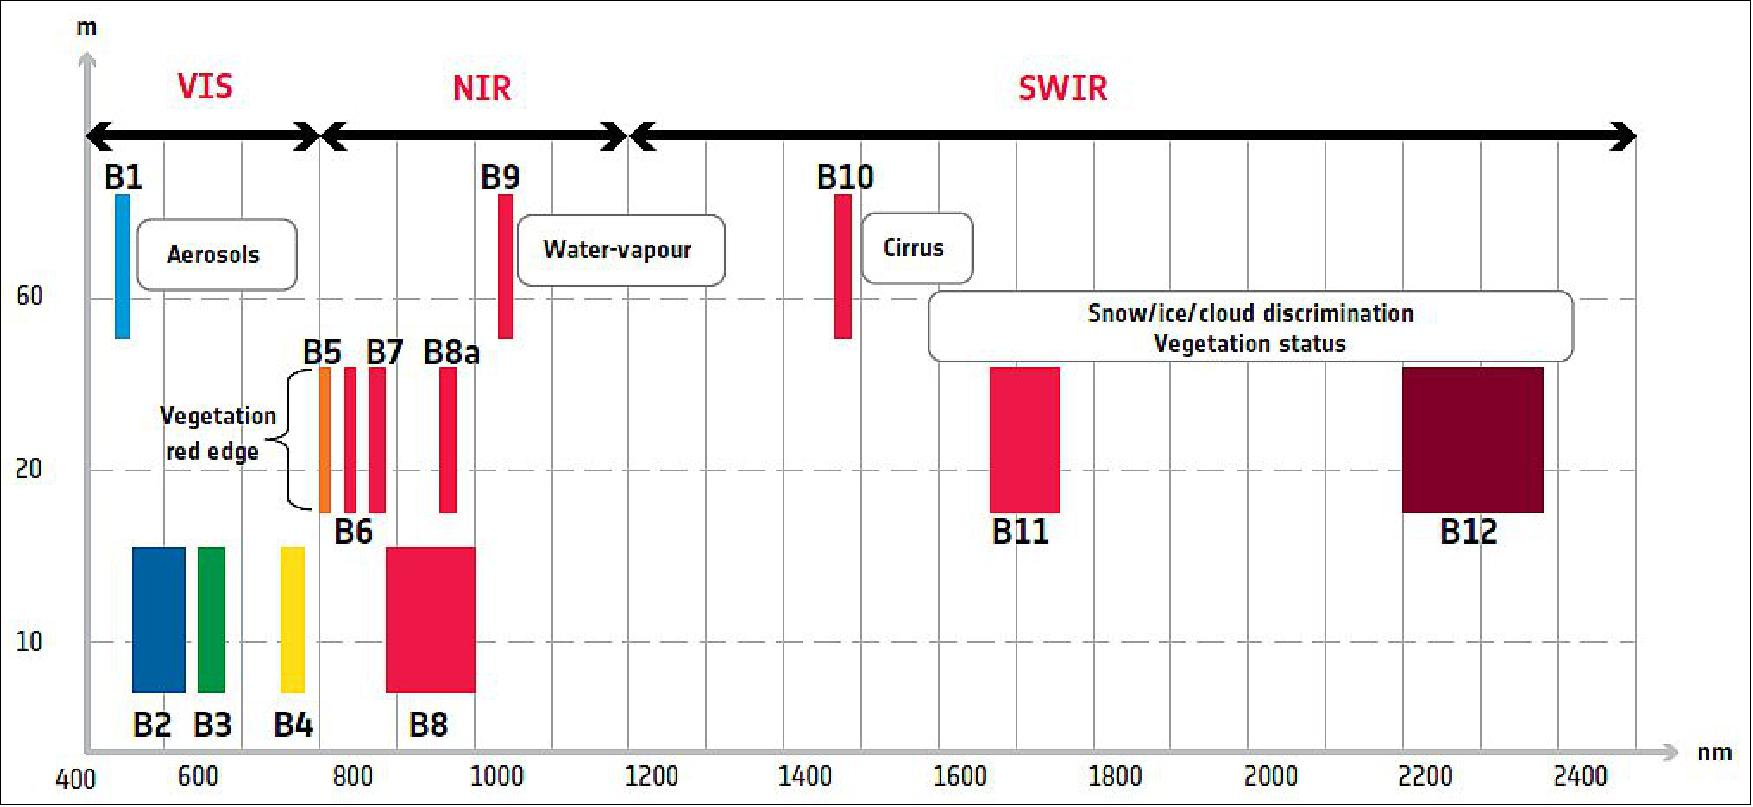
\includegraphics[width=0.4\textwidth]{satelite/sentinel-2-bands.jpg}
							% 	\caption{XXX Sentinel 2 bands}
							% \end{figure}
			Additional to the spectral bands, the ESA also supplies a Scene Classification Layer (\textit{SCL})\todo{Hier noch erwähnen, dass die SCL das Resultat eines Algorithmus der ESA ist. Das kann in der Diskussion dann auch wieder aufgenommen werden \& kritisch hinterfragt werden.} where for each location the observed subject is assigned to an \textit{SCL-class} (cf. table~\ref{tab:satelite/scl_classes}). In chapter \ref{sec:itpl}  we will use this classification to filter out unreliable data points, considering only SCL-classes 4 and 5.  
			
			
			\begin{table}[h]
				\caption{Overview: Scene Classification Layers (SCL)}
				\label{tab:satelite/scl_classes}
				\center
				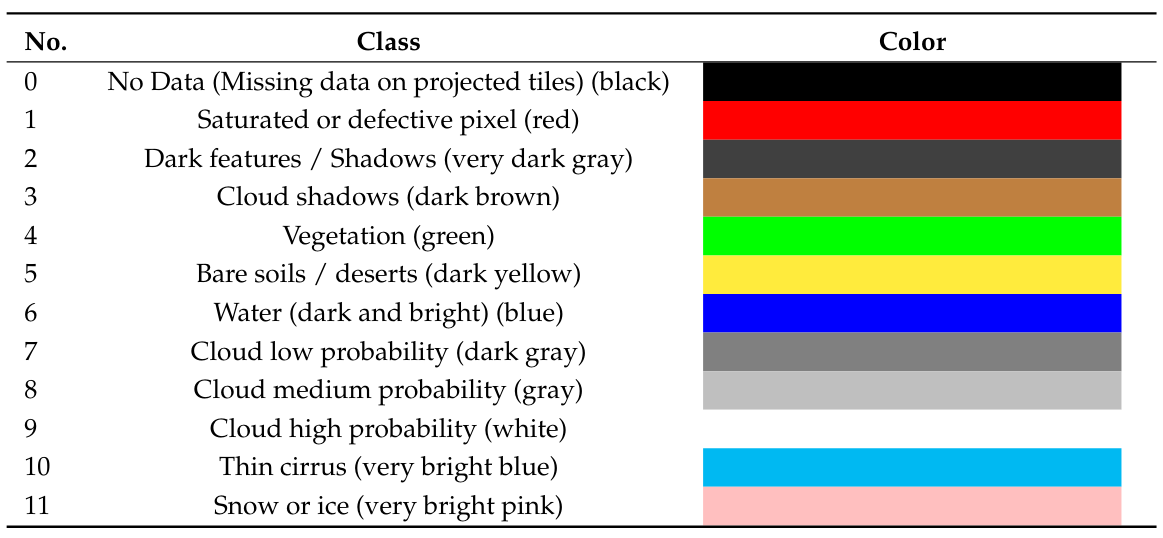
\includegraphics[width=0.8\textwidth]{satelite/scl_classes.png}
			\end{table}
		}

		\subsubsection*{Data Illustration XXXorXXX Challenges in S2 Data}{
				%satelite/time_series_2021_P112/15_scl5_2021-02-23.png
	%satelite/time_series_2021_P112/30_scl4_2021-05-09.png
	%satelite/time_series_2021_P112/33_scl9_2021-05-24.png
	%satelite/time_series_2021_P112/35_scl4_2021-06-03.png
	%satelite/time_series_2021_P112/40_scl10_2021-06-28.png
	%satelite/time_series_2021_P112/45_scl2_2021-07-23.png

\begin{figure*}
	\centering
	\begin{subfigure}[b]{0.31\textwidth}
		\centering
		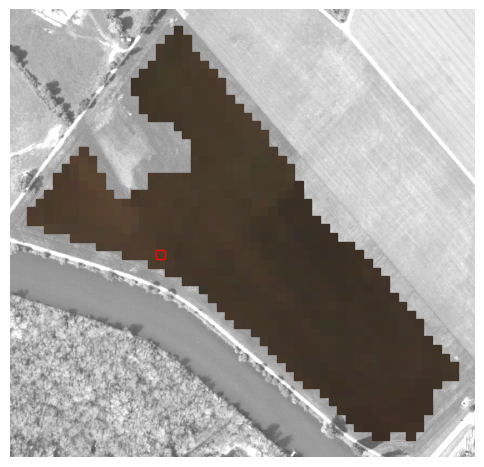
\includegraphics[width=\textwidth]{satelite/time_series_2021_P112/15_scl5_2021-02-23.png}
		\caption[2021-02-23\hspace*{0.1cm} SCL 5]%
		{{\small 2021-02-23\hspace*{0.1cm} SCL 5}}    
		\label{fig:satelite/time_series_2021_P112/15_scl5_2021-02-23.png}
	\end{subfigure}
	\hfill
	\begin{subfigure}[b]{0.31\textwidth}  
		\centering 
		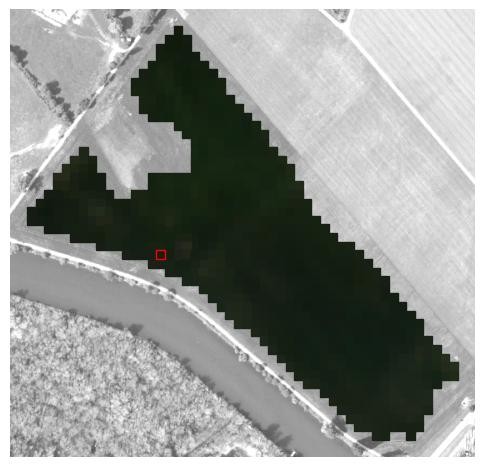
\includegraphics[width=\textwidth]{satelite/time_series_2021_P112/30_scl4_2021-05-09.png}
		\caption[2021-05-09\hspace*{0.1cm} SCL 4]%
		{{\small 2021-05-09\hspace*{0.1cm} SCL 4}}    
		\label{fig:satelite/time_series_2021_P112/30_scl4_2021-05-09.png}
	\end{subfigure}
	\hfill
	\begin{subfigure}[b]{0.31\textwidth}  
		\centering 
		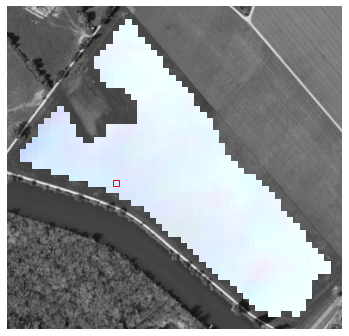
\includegraphics[width=\textwidth]{satelite/time_series_2021_P112/33_scl9_2021-05-24.png}
		\caption[2021-05-24\hspace*{0.1cm} SCL 9]%
		{{\small 2021-05-24\hspace*{0.1cm} SCL 9}}    
		\label{fig:satelite/time_series_2021_P112/33_scl9_2021-05-24.png}
	\end{subfigure}

	\vskip\baselineskip
	\begin{subfigure}[b]{0.31\textwidth}   
		\centering 
		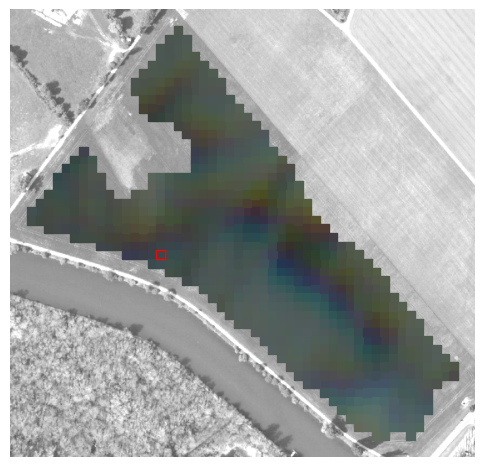
\includegraphics[width=\textwidth]{satelite/time_series_2021_P112/35_scl4_2021-06-03.png}
		\caption[2021-06-03\hspace*{0.1cm} SCL 4]%
		{{\small 2021-06-03\hspace*{0.1cm} SCL 4}}    
		\label{fig:satelite/time_series_2021_P112/35_scl4_2021-06-03.png}
	\end{subfigure}
	\hfill
	\begin{subfigure}[b]{0.31\textwidth}   
		\centering 
		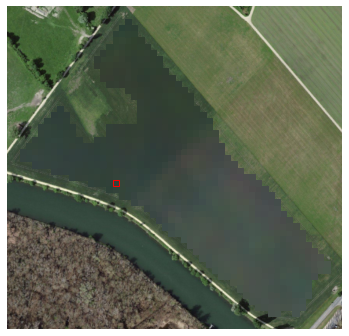
\includegraphics[width=\textwidth]{satelite/time_series_2021_P112/40_scl10_2021-06-28.png}
		\caption[2021-06-28\hspace*{0.1cm} SCL 10]%
		{\small 2021-06-28\hspace*{0.1cm} SCL 10}    
		\label{fig:satelite/time_series_2021_P112/40_scl10_2021-06-28.png}
	\end{subfigure}
	\hfill
	\begin{subfigure}[b]{0.31\textwidth}  
		\centering 
		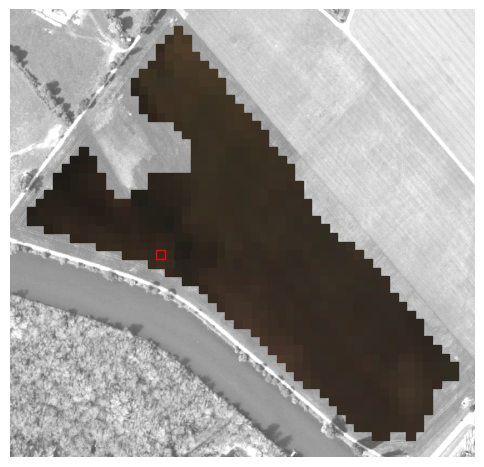
\includegraphics[width=\textwidth]{satelite/time_series_2021_P112/45_scl2_2021-07-23.png}
		\caption[2021-07-23\hspace*{0.1cm} SCL 2]%
		{{\small 2021-07-23\hspace*{0.1cm} SCL 2}}    
		\label{fig:satelite/time_series_2021_P112/45_scl2_2021-07-23.png}
	\end{subfigure}

	\vskip\baselineskip
	\begin{subfigure}[b]{0.7\textwidth}   
		\centering 
		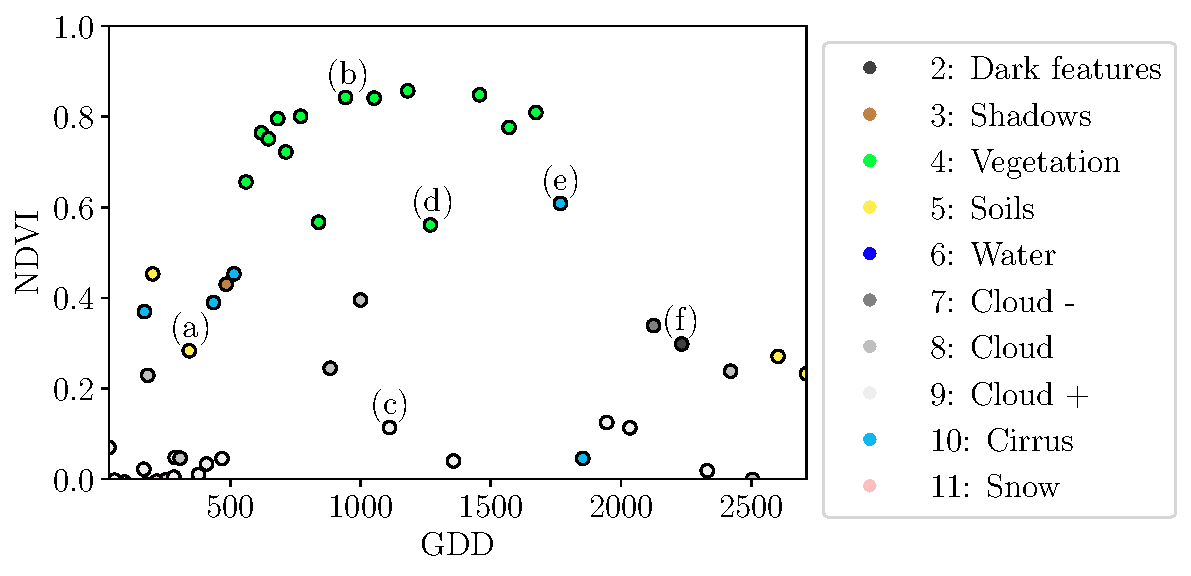
\includegraphics[width=\textwidth]{interpol/ndvi_ts_scl.pdf}
		\caption[Corresponding NDVI {TS}]%
		{{\small Corresponding NDVI {TS}}}    
		\label{fig:interpol/ndvi_ts_scl45_grey.pdf}
	\end{subfigure}
	\vspace{0.3cm}
	\caption[Satellite images of a field at selected times + NDVI TS]{Satellite images of a field at selected times with a static grayscale background for orientation. Moreover, the NDVI {TS} of the red-highlighted pixel is shown in (g) colored by the SCL labels.} 
	\label{fig:witzwil_selected_satellite_images}
\end{figure*}


\todo{Hier noch eine NDVI Zeitreihe parallel dazu zeigen. Ansonsten wird nicht klar, warum wir die Interpolation überhaupt machen.}
			% Description of plot
			The figure ~\ref{fig:witzwil_selected_satellite_images} shows a selection of 6 satellite images of a field, which display our challenges\todo{which challenges? were they introduced earlier? E.g. in the introduction?}. In February (image a), we see no vegetation but bare soil. At the beginning of May, we observe a cloudless dark green field. In (c) heavy cloud cover (SCL class 9) leads to a complete loss of plant information in this S2 observation. Figure (d) shows that the SCL classification is not reliable, since we evidently observe clouds. In (e) we see a pale green. This likely shimmers through cirrus clouds. 
			
			%% subfigures references:
			% (see. \ref{fig:satelite/time_series_2021_P112/15_scl5_2021-02-23.png})
			% (see. \ref{fig:satelite/time_series_2021_P112/30_scl4_2021-05-09.png})
			% (see. \ref{fig:satelite/time_series_2021_P112/33_scl9_2021-05-24.png})
			% (see. \ref{fig:satelite/time_series_2021_P112/35_scl4_2021-06-03.png})
			% (see. \ref{fig:satelite/time_series_2021_P112/40_scl10_2021-06-28.png})
			% (see. \ref{fig:satelite/time_series_2021_P112/45_scl2_2021-07-23.png})
		}
	}

	\subsection{Crop Yield Data}\todo{Hier bitte noch eine kleine Beschreibung der Crop-yields reinnehmen. Also was sind die Ertragswerte der Daten.}{
		\label{sec:yieldmapping_data}
		The crop yield data were collected using a combine harvester. Equipped with GPS, the harvester drives over the fields and continuously estimates the crop density in $t/ha$ (see fig. \ref{fig:satelite/witzwil_2021_P112_yield_harvester_cropped}). 
		We take the data set derived from this in REF-Gregor-Perich, where error-prone measurement points (such as during a tight curve of the combine harvester) were removed and then the yield map was rasterized using linear interpolation (cf. fig. \ref{fig:satelite/witzwil_2021_P112_yield_cropped.png}).    

		
		Comparing the average per-field crop yield reported by the farmer with the yield estimated by the combine harvester shows that the latter overestimates crop yield by ca. $10\%$ (cf. REF-gregor). Since the relative estimation error is approximately constant and we do not aim to estimate the absolute yield, we will not consider this deviation.
		\begin{figure}
			\centering
			\begin{subfigure}{.5\textwidth}
			  \centering
			  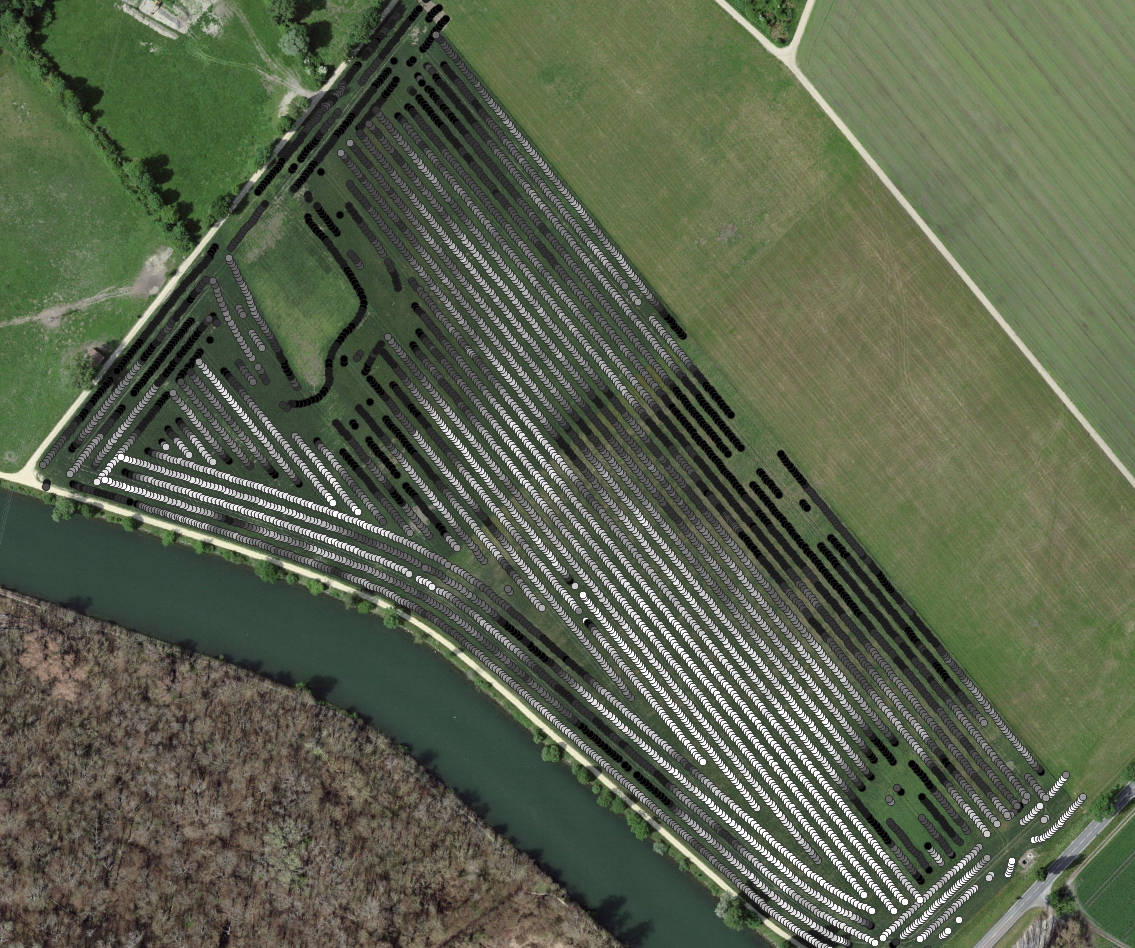
\includegraphics[height=.75\linewidth]{satelite/witzwil_2021_P112_yield_harvester_cropped.png}
			  \caption{Raw combine harvester data (cleaned)}
			  \label{fig:satelite/witzwil_2021_P112_yield_harvester_cropped}
			\end{subfigure}%
			\begin{subfigure}{.5\textwidth}
				\centering
				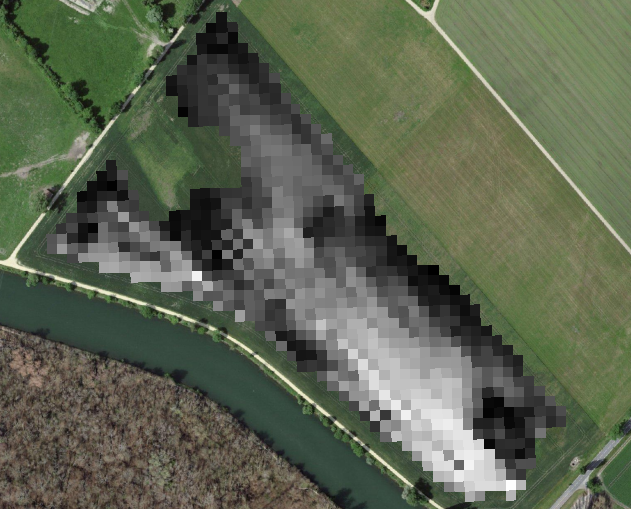
\includegraphics[height=.75\linewidth]{satelite/witzwil_2021_P112_yield_cropped.png}
			  \caption{rasterized to Sentinel 2 resolution.}
			  \label{fig:satelite/witzwil_2021_P112_yield_cropped.png}
			\end{subfigure}
			\caption{Crop yield density map of a field. Ranges from 0.1 t/ha (black) to 5.35 t/ha (white) }
			\label{fig:satelite_witzwil_yield}
		\end{figure}
	}


	\subsection{The Concept of a `Pixel'}{
		\label{sec:gather_data_to_pixel}
		Before we join all the data, we define a few concepts.

		{% NDVI
			The well-known Normalized Difference Vegetation Index (\textit{NDVI}) introduced in \cite{rouseMonitoringVernalAdvancement1974} can be calculated using the bands $B4$ and $B8$ (table \ref{table:S2-bands}) by:
			\begin{equation}
				NDVI = \frac{B8 - B4}{B8 + B4}
				\label{eq:ndvi}
			\end{equation}
			Note that we call the calculated values merely the \textit{observed NDVI}, as we must be aware of imprecisions due to clouds and shadows\todo{Please clarify this in more detail. We used pixels flagged with SCL 4 \& 5, but as can be seen in Fig. 2.1 d), this can yield erroneous NDVI values, etc.}. 
		}

		{% GDD & DAS
			To define a timescale, we consider Days After Sowing (\textit{DAS}) and a transformed timescale, Growing Degree Days (\textit{GDD}) (\cite{mcmasterGrowingDegreedaysOne1997}REF). The latter are defined as the cumulative sum (since sowing) of temperature above a given base temperature $T_{base}$. For cereals, we use $T_{base}=0$ (REF-Gregor). Thus, the GGD for $n$ days after sowing will be equal to:\todo{Für den Leser wäre es interessant, wenn Du noch kurz die wichtigsten GDD Werte aus der Literatur beschreiben würdest (D.h. z.B. Sowing, Emergence of Plants, Anthesis, Senescence, Harvest)}
			\begin{equation}
				\label{eq:gdd}
				GDD_n := \sum_{i=0}^n \max(T_i - T_{base}, 0).
			\end{equation}
		} 

		Now we create a data set, which will contain all the necessary information\todo{necessary info for what? To answer the research questions asked in section XXX}. Given that we have the spectral data at a $10m \times 10m$ resolution, we introduce the concept of a Pixel. A \textit{Pixel} $P$ is associated with a $10m \times 10m$ square defined by the S2 satellites and contains all relevant information\todo{which?} for a season and this location. More precisely, $P$ is a collection of general information (like yield and coordinates) and all associated $P_t$ of a given season. Where $P_t$ represents a tuple of the spectral data for time $t$, the NDVI calculated from it, and the associated GDD. 
		We will call the resulting data set \textit{PIXELS}, as it is the collection of all Pixels (over all seasons). 
		
		% Finally, we split PIXELS randomly into a train ($80\%$) and test  ($20\%$) set. 

	}

\section{General Methods}{
	We will only introduce general methods within this section, whereas more specific methods will be introduced in their context\todo{which context? I would write: "... introduced in chapter/section XXX in more detail.}. We discuss interpolation methods in sections \ref{sec:itpl_parametric} and \ref{sec:itpl_nonparametric}, a robustification strategy in section \ref{sec:loess_robustify}, a method how we can objectively determine the quality of an interpolation in section \ref{sec:itpl_param_est}, and in section \ref{sec:corr_correction} we present the NDVI correction with an adapted interpolation strategy.


	\subsection{(Relative) RMSE}
		\todo[inline]{definithion here and also relative}

	\subsection{Out-Of-Bag (\textit{OOB}) and Leave-One-Out-Cross-Validation (\textit{LOOCV})}{
	    \todo[inline]{Hier fehlt mir eine kurze Erklärung, was OOB und LOOCV sind.}
		\label{sec:OOB_LOOCV}
		Let 
		$$
			D=\{(X_{[j,:]},y_j)|\; X\in\R^{n\times p}, y\in \R^n, j=1,\dots,n\}
		$$
		be a dataset, $i\in \{1,\dots,n\}$ and $M^{(-i)}$ a model fitted on a subset of $D\setminus\{(X_{[i,:]},y_i)\}$. Then we call $\hat y_i:= M^{(-i)}(X_{[i,:]})$ an \textit{OOB} estimator of $y_i$. If we do this for all $i\in\{1,\dots,n\}$, we obtain $\hat y := \left(\hat y_1,\dots,\hat y_n\right)$ the OOB estimator for $y\in \R^n$.

		In the bootstrap (e.g., random forest) framework, we define $\hat y_i$ to be the average of all computed and admissible $M^{(-i)}$. 
		
		In the case that $M^{(-i)}$ was fitted on the set $D\setminus\{(X_i,y_i)\}$ (i.e., not a true subset), we call the corresponding $\hat y_i$ also the LOOCV estimator.	

		If we optimize some parameter via OOB (or LOOCV) this means that we search for the parameter that minimizes some loss function which takes the OOB (or LOOCV) residuals. Usually we approximate this parameter by searching on a grid. 
	}

	\subsection{Generalized Cross Validation (GCV)}{
		\todo[inline]{definition here and explanation why (computational cheap)}

	}
}
